\chapter{MVC in IBM Content Navigator}
\label{chap:nexus}
This chapter introduces the IBM Content Navigator application and framework. After an overview on its architecture and plugin system, the main client-side components Dojo and \ac{idx} are outlined. To conclude this chapter, the design and implementation of a log analysis plugin is discussed.
\section{Architecture and Extension Points}
% IBM Content Navigator is an enterprise web application written in Java and JavaScript. It is designed to run on a \ac{j2ee} application server

\subsection{Architecture: Layers and Components}
\nexus\ is designed after the \emph{Separation of Concerns} principle. It consists of different layers which are shown in Figure~\ref{fig:nexuslayers}

\begin{figure}[H]
	\centering
	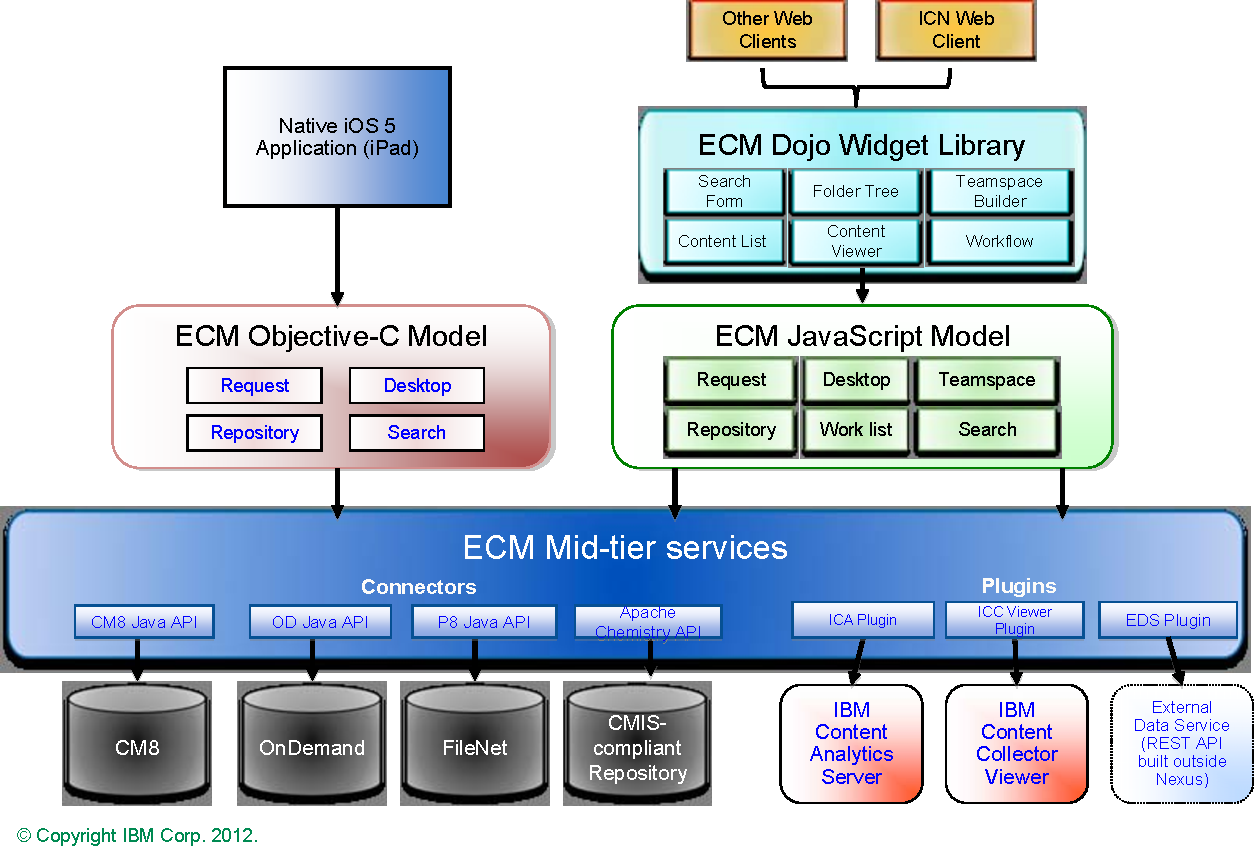
\includegraphics[width=14cm]{images/nexuslayers.pdf}
	\caption{Layers of IBM Content Navigator}
	%\captionsetup{font={footnotesize,bf,it}}
	%\caption*{Source: \cite[p. 5]{gof}}
	\label{fig:nexuslayers}
\end{figure}

The top layer represents the actual clients for Content Navigator. Besides the desktop web client, there are also mobile and an iOS 5 client. The client layer makes use of the widget layer underneath that contains all the Dojo widgets (\emph{Dijits}). In turn, the widgets access the modelling layer, which contains JavaScript Models held in the browser. On the one hand, these models can be connected to mid-tier services, such as ECM repository \glspl{api}, on the other hand, they can be directly connected to a external, HTTP-based services, such as \ac{rest}.

The mid-tier services are implemented in Java and run on the application server, whereas the modelling and widget layers run in the browser. This is illustrated by Figure~\ref{fig:nexustiers}, which shows the tier architecture of Content Navigator.

\begin{figure}[H]
	\centering
	\includegraphics[width=14cm]{images/nexustiers.pdf}
	\caption{3-Tier architecture of IBM Content Navigator}
	%\captionsetup{font={footnotesize,bf,it}}
	%\caption*{Source: \cite[p. 5]{gof}}
	\label{fig:nexuslayers}
\end{figure}

\subsection{Extension Points: Plug-ins}
The modular architecture presented before makes it easy to extend \nexus\ on different levels.

\subsubsection{Actions}
\subsubsection{Services}
\subsubsection{Features}

% TODO: muss es DB2 sein? wie wird das eingestellt?
\subsection{Deployment and Configuration}
Content Navigator itself is packaged --- without any plug-ins --- into an \ac{ear} file and can directly be deployed on an application server, such as IBM \acl{was}. The connection to a DB2 database for storing and loading the configuration is needed and can be set up using the \ac{jre} environment variables.

Plug-ins are deployed seperately. They are packaged as \ac{jar} files and can be loaded using the Administration Desktop of \nexus. This allows the application administrator to update, load and unload plug-ins without restarting \nexus\ or the application server.

\section{Dojo (and IDX) MVC} % brauche ich IDX hier wirklich?
This section introduces the components of Dojo that are relevant to building \acl{mvc} applications, and those that were especially used while building the log analysis plugin for \ac{sccm}. As IBM Content Navigator 2.0 (which is the latest version as of August 2012) includes Dojo 1.6, this is the version of Dojo referred here.

\subsection{Dojo Basics}
The Dojo Toolkit, usually just called \emph{Dojo}, is a set of libraries to build JavaScript applications. In opposite to other JavaScript libraries, such as jQuery, Prototype or Mootools, Dojo is not only aimed at simplifying \ac{dom} manipulation, \ac{ajax} and event handling, but also comes with an extensive widget library (\emph{Dijit}) and charting \ac{api}.

Dojo is separated into three packages:
\begin{description}
	\item[Dojo] is the core package and contains basic functionality, such as \ac{dom} manipulation, \ac{ajax}, effects, and JavaScript language helpers. Its namespace is \code{dojo}.
	\item[Dijit] contains all stable widgets, such as layout widgets, forms, dialogs, and a tree view. Its namespace is \code{dijit}.
	\item[DojoX] are the Dojo extensions in the namespace \code{dojox}. This package contains less common components, such as the graphing and charting \ac{api}. The DojoX Grid (\code{dojox.grid.DataGrid}) and the JsonRestStore (\code{dojox.data.JsonRestStore}) are further discussed in Section~\ref{sec:loganal}.
\end{description}

JavaScript is a prototype-based object-oriented programming language. Dojo simulates class-based object orientation, which is more familiar to developers used to Java, C++, C\# and other languages. Listing~\ref{lst:classes} contains the declaration of a Dojo class using \code{dojo.declare} for illustration.

\begin{listing}[H]
\begin{minted}[linenos=true,frame=no]{javascript}
dojo.declare("my.Thinger", null, {
  constructor: function(/* Object */args){
    dojo.safeMixin(this, args);
  }
});
\end{minted}
\caption{Declaring a Dojo class}
\label{lst:classes}
\end{listing}

This listing declare the \code{my.Thinger} class (in the \code{my} namespace). When instantiating an object, the constructor does nothing else than mixing the \code{args} argument, which should be a JavaScript object, into the new instance. This is shown in Listing~\ref{lst:mixin}.

\begin{listing}[H]
\begin{minted}[linenos=true,frame=no]{javascript}
var thing = new my.Thinger({ count:100 });
console.log(thing.count);
\end{minted}
\caption{Instantiating an object using a Dojo class}
\label{lst:mixin}
\end{listing}

The object\footnote{JavaScript objects can simply be created as literals. Object literals are enclosed in braces (`\{' and `\}') and contain a comma-separated list of properties (attributes and methods).} provided as an argument to the \code{my.Thinger()} constructor is mixed into the new object \code{thing}. This means, that \code{thing} now contains the properties of this object, which can be proven by printing out \code{thing.count} in the console.

All Dojo components, including Dijits, are created using this concept, and so are the classes developed for the log analysis plug-in.

Another of Dojo's concepts being of help in \ac{mvc} applications and the plug-in is \code{dojo.hitch}. The JavaScript \ac{api} of web browsers features a callback-based event system. This means that callbacks are registered to an event and triggered when the event occurs. A frequently faced problem\footnote{\placeholder{quelle hierfür}} is that the callback function has a different scope than the function that defines the callback. In JavaScript, this is typically solved using a \emph{closure}, a concept to pass on a given scope to another function. In applications with a lot of callbacks, which may also be depending on each other to execute, closures can get confusing. \code{dojo.hitch} returns a function that, when executed, has a specified scope, as shown in Listing~\ref{lst:hitch}.

\begin{listing}[H]
\begin{minted}[linenos=true,frame=no]{javascript}
function myCallback() {
  console.log(this.localVariable)
}

dojo.declare("my.Thinger", null, {

  localVariable: "I am in the Thinger scope",
  button: null,

  constructor: function() {
    this.button = new dijit.form.Button({
      label: "Hello"
    });
    dojo.connect(this.button, 'onClick', dojo.hitch(this, myCallback));
  }
});

var thing = new my.Thinger();
\end{minted}
\caption{Instantiating an object using a Dojo class}
\label{lst:hitch}
\end{listing}

This listing first defines a function that acts as a callback and refers a variable (``localVariable'') of its own scope (``this''). The Dojo class declared below introduces said variable and constructs a button.

\subsection{MVC Components}

%=============================================================================
%=============================================================================

\section{Implementation of a Log Analysis Plugin}
\label{sec:loganal}
In the context of this Bachelor's thesis, a log analysis system was developed by two students. The author created a front-end using \ac{ibm} \nexus, whereas Robert Metzger implemented the respective back-end using \ac{ibm} BigInsights.
\subsection{Motivation}
\ac{ibm} \acl{sccm} is a \acl{saas} to cover use cases of \acl{ecm}. It is a large integration project that makes use of many IBM software products, such as DB2\footnote{IBM DB2 is a relational database management system (DBMS).}, FileNet P8, \acl{was} and Content Collector\footnote{\placeholder{todo}}, to provide an out--of--the--box content management solution to customers. In this environment, massive amounts of operational data are generated, especially if multiple customers are involved.

As \ac{ibm} is responsible for the operation of \ac{sccm}, problems have to be solved immediately as they arise, and steps must be taken to prevent problems beforehand. The large amounts of log data that the integrated software products generate contain knowledge that is necessary for \emph{predictive analysis}. Using IBM BigInsights, related and correlated log entries can be found and integrated to gain insights on the system's state and arising problems. % evtl noch die log-level geschichte ansprechen

These analysis results have to be made available to the cloud operator in an easily accessable manner. Using \nexus\ to develop a front-end for the log analysis system not only makes it possible to integrate it with any \nexus based product, but also emphasizes its ability to serve as a flexible, versatile web application framework.

The design and implementation of the BigInsights back-end are not in the scope of this thesis, as they mostly reflect the work of Robert Metzger. Nevertheless the interface to the back-end --- a \ac{rest} service --- will be presented, as it is essential to some functionality of the front-end.
% Developing a front-end for the log analysis system using \nexus\ not only makes it possible to integrate it with any \nexus\ based product, but also emphasizes its ability to 
% predictive analysis
\subsection{Design}
\subsection{Implementation}